\documentclass[pdflatex,sn-mathphys-num]{sn-jnl}

\usepackage{graphicx}
\usepackage{amsmath,amssymb,amsfonts}
\usepackage{booktabs}
\usepackage{array}
\usepackage{url}
\usepackage{tikz}
\usetikzlibrary{arrows.meta,positioning,shapes.geometric}

\raggedbottom
\hypersetup{bookmarksdepth=2}

\begin{document}

\title[Full-GPU PH-SHOWOA]{A Full-GPU PH-SHOWOA with SA-RCRS-GRASP Initialization for VRPSPDTW}

\author[3]{\fnm{Huynh Khang} \sur{Lam}}\email{khanglhse200666@fpt.edu.vn}
\author[3]{\fnm{Anh Huy} \sur{Bui}}\email{huy@fpt.edu.vn}
\author*[1,2,3]{\fnm{Tri Minh} \sur{Pham}}\email{tri.phamhpc@hcmut.edu.vn}

\affil*[1]{\orgname{Ho Chi Minh City University of Technology (HCMUT)}, \orgaddress{\city{Ho Chi Minh City}, \country{Vietnam}}}
\affil[2]{\orgname{Vietnam National University, Ho Chi Minh City}, \orgaddress{\city{Ho Chi Minh City}, \country{Vietnam}}}
\affil[3]{\orgdiv{AiTA Lab, Faculty of Information Technology}, \orgname{FPT University}, \orgaddress{\city{Ho Chi Minh City}, \country{Vietnam}}}

\abstract{The Vehicle Routing Problem with Simultaneous Pickup and Delivery and Time Windows (VRPSPDTW) is difficult because every route must satisfy capacity and time-window constraints while the number of vehicles is minimized before travel distance. PH-SHOWOA is a parallel hybrid of the Spotted Hyena Optimizer (SHO) and Whale Optimization Algorithm (WOA). Its original implementation was designed for CPU execution. This paper presents fullGPU-SA-RCRS-GRASP, a Python CUDA implementation that keeps the solution population, route data, objective values, random states, and search operators on the GPU during a run. The original simulated-annealing initialization is replaced by an SA-RCRS-GRASP construction that uses a restricted candidate list and a short simulated-annealing warm-up. The implementation uses fixed-shape tensors and preallocated device buffers, so it avoids CPU--GPU synchronization inside the search loop. On 15 Wang--Chen benchmark instances, the GPU implementation preserves the number of vehicles on 14 instances and improves it on one instance. It obtains equal or shorter total distance on 14 instances. The aggregate runtime falls from 104,175 s to 3,648.2 s, which is a 28.6-fold speedup for the reported experiment. These results show that a GPU-resident design can greatly reduce runtime while maintaining competitive routing quality.}

\keywords{VRPSPDTW, GPU computing, metaheuristic, PH-SHOWOA, SA-RCRS-GRASP, CUDA}

\maketitle

\section{Introduction}\label{sec:intro}

The vehicle routing problem with simultaneous pickup and delivery and time windows (VRPSPDTW) asks for a set of routes that serve all customers. A vehicle may deliver goods and collect goods at the same customer, and every service must respect its time window and the vehicle capacity. Following the original PH-SHOWOA paper, reducing the number of vehicles (NV) is the primary objective because it has a large fixed operating cost. Total distance (TD) is compared only after NV.

The VRPSPDTW extends classical time-window routing \cite{solomon1987algorithms,laporte2009fifty} by requiring simultaneous delivery and pickup. Its model, practical instances, exact methods, and multiobjective variants have been studied in several forms \cite{angelelli2002vrpspdtw,wang2015multiobjective,praxe2024exact}. The VRPSPDTW has also been studied with genetic algorithms, parallel simulated annealing, adaptive large-neighborhood search, lexicographic two-stage search, and memetic search \cite{wang2012ga,wang2015psa,hof2019alns,shi2020lexicographic,liu2021memetic,lei2025memetic}. These studies support the use of a hierarchical objective: minimize NV first and then TD \cite{wang2015psa,shi2020lexicographic}. Recent studies show the value of local search, hybridization, and multi-stage search when pickup, delivery, capacity, and time windows interact \cite{wu2023aco,liu2023hybrid,zhang2025multistage,mu2016parallel,voigt2025alns}. PH-SHOWOA combines the exploration behaviour of the Spotted Hyena Optimizer (SHO) with the best-guided intensification of the Whale Optimization Algorithm (WOA) \cite{dhiman2017sho,mirjalili2016woa,gharehchopogh2019woasurvey,utama2023hsho,zhou2024whalerouting,nguyen2026phshowoa}. The original work also uses simulated annealing, local search, diversification, and parallel solution updates. Although these components produce good routes, route construction, feasibility checks, and population updates create many small computations. A conventional CPU-oriented implementation cannot fully use the large parallel capacity of a modern GPU.

GPU computing provides a natural way to evaluate and update many population members at once. CUDA was designed for scalable parallel execution of data-parallel workloads \cite{nickolls2008cuda}, while recent tensorized evolutionary optimization shows that candidate populations, objective values, and variation operators can be reformulated as dense device tensors \cite{liang2026tensorization}. GPU acceleration has also been investigated for metaheuristic benchmarking and vehicle-routing local optimization \cite{dorneles2023gpu,lin2025tensorvrp}. Parallel portfolio construction gives another useful view of distributing diverse search behavior across concurrent workers \cite{tang2021portfolio}. However, accelerating only route evaluation still leaves repeated host-device transfers and CPU-side search control as sources of overhead. This work develops a full-GPU version of PH-SHOWOA in Python. The proposed method changes the initial construction to SA-RCRS-GRASP and performs the full search of one run on the GPU. CPU work is limited to preparing immutable instance data and decoding the final best solution after all runs. The main aim is to reduce runtime without changing the NV-first priority of the original method.

The research gap is therefore not only a faster route evaluator, but a complete PH-SHOWOA search procedure that stays on the GPU. The present work addresses this gap through a GPU-resident population representation, a GPU implementation of SA-RCRS-GRASP initialization, and device-side search and repair operators. The evaluation examines whether this design reduces runtime while preserving the original NV-first routing objective. The source code, benchmark inputs, and scripts are publicly available at \url{https://github.com/Welkie/ph-showoa}.

\section{Materials and methods}\label{sec:methods}

\subsection{Datasets}\label{sec:datasets}

The study uses Wang--Chen VRPSPDTW benchmark instances recorded in the project repository \cite{wang2012ga}. They include random (Rdp), clustered (Cdp), and mixed random--clustered (RCdp) customer layouts. Each instance specifies customer delivery and pickup demand, service time, capacity, time windows, and distance and travel-time matrices. The reported experiment contains 15 instances: one instance with 10 customers, three with 50 customers, and eleven with 100 customers. These varied layouts make it possible to examine both small and medium-size routing cases.

\subsection{Problem formulation and baseline framework}\label{sec:problem}

Let $V=\{0,1,\ldots,n\}$ be the depot and $n$ customers. Each customer has delivery demand, pickup demand, service time, and a time window. A feasible route begins and ends at the depot, visits each customer exactly once over all routes, and respects the time and capacity constraints at every route position. The solution quality is compared lexicographically: a solution with fewer vehicles is always preferred; only when two solutions use the same number of vehicles is the shorter TD preferred. For implementation, the same preference is represented by the scalar score
\begin{equation}
 F(S)=2000\,NV(S)+TD(S),
\label{eq:fitness}
\end{equation}
where the large vehicle weight makes the search prefer a vehicle reduction before a distance reduction.

The baseline PH-SHOWOA alternates SHO-like population diversification and WOA-like intensification around the current best solution \cite{nguyen2026phshowoa}. It also applies simulated-annealing acceptance and periodic route improvements. This work retains this search principle, but redesigns the data and operators for a GPU-resident execution.

\subsection{Proposed full-GPU PH-SHOWOA method}\label{sec:method}

Figure~\ref{fig:phshowoa-flow} gives the algorithmic flow of the proposed PH-SHOWOA. It retains the SHO/WOA hybrid search of the original method, but replaces the original initial-population step with SA-RCRS-GRASP. Every acceptance and best-solution comparison follows the NV-first, TD-second rule. The flow is algorithmic; Figure~\ref{fig:workflow} separately shows where CPU and GPU execution occur.

\begin{figure*}[t]
\centering
\resizebox{\textwidth}{!}{%
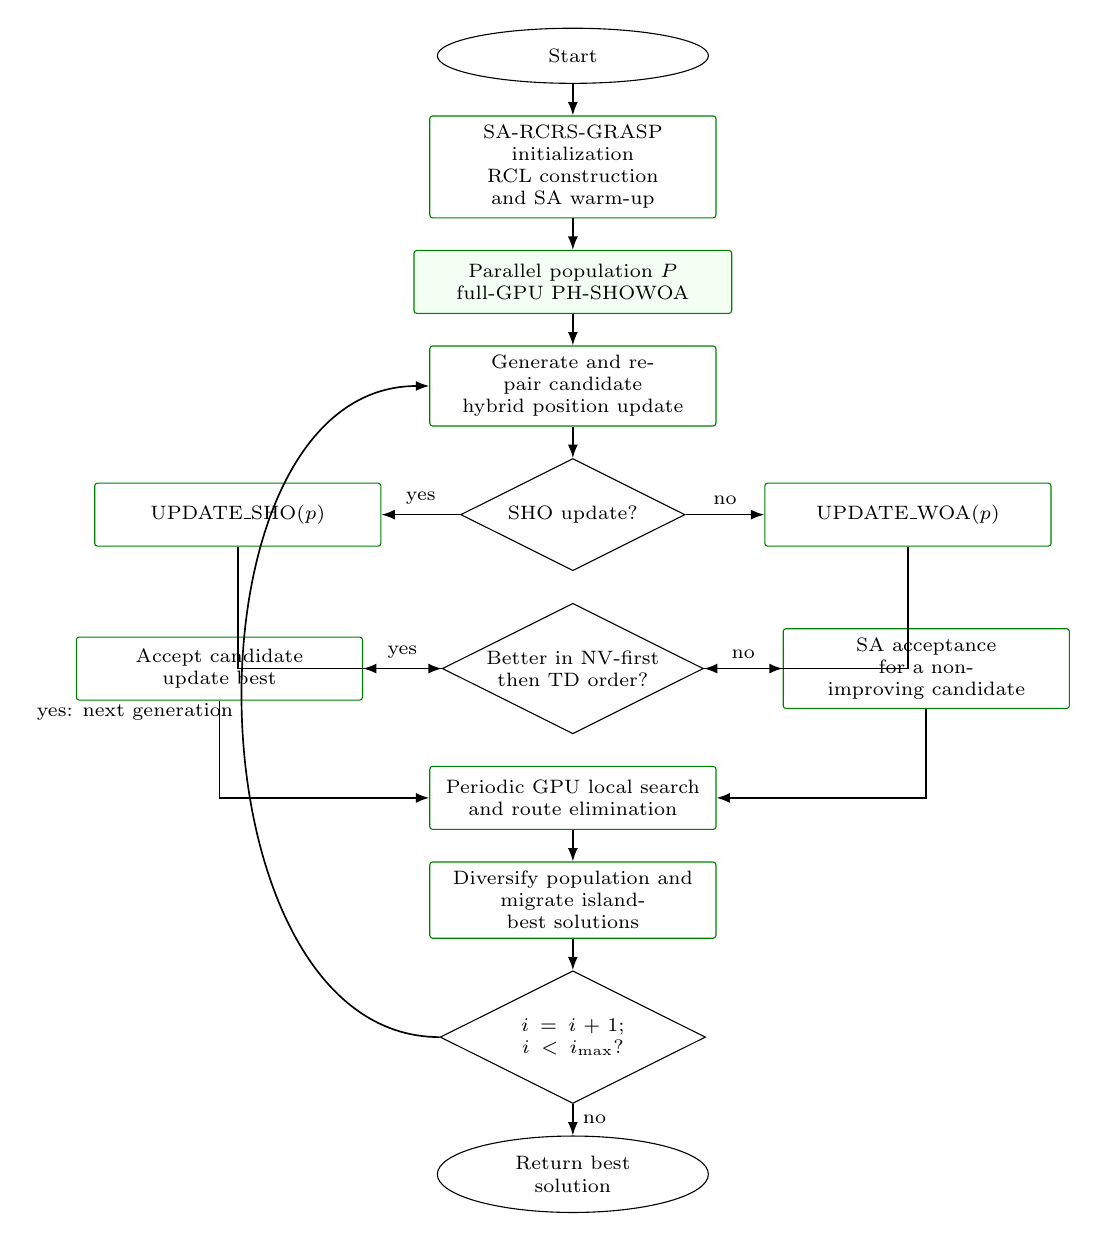
\begin{tikzpicture}[font=\scriptsize, node distance=4mm and 10mm,
  process/.style={draw=green!50!black, rounded corners=1pt, align=center, minimum height=8mm, text width=34mm},
  decision/.style={draw, diamond, aspect=2.0, align=center, inner sep=1pt, text width=22mm, minimum height=11mm},
  terminal/.style={draw, ellipse, align=center, minimum height=7mm, text width=22mm},
  hybrid/.style={draw=green!50!black, rounded corners=1pt, align=center, fill=green!5, minimum height=8mm, text width=38mm},
  flow/.style={-{Latex[length=1.7mm]}, semithick}]
\node[terminal] (start) {Start};
\node[process, below=of start] (initial) {SA-RCRS-GRASP initialization\\RCL construction and SA warm-up};
\node[hybrid, below=of initial] (population) {Parallel population $P$\\full-GPU PH-SHOWOA};
\node[process, below=of population] (candidate) {Generate and repair candidate\\hybrid position update};
\node[decision, below=of candidate] (hybridcheck) {SHO update?};
\node[process, left=of hybridcheck] (sho) {UPDATE\_SHO$(p)$};
\node[process, right=of hybridcheck] (woa) {UPDATE\_WOA$(p)$};
\node[decision, below=of hybridcheck] (better) {Better in NV-first\\then TD order?};
\node[process, left=of better] (accept) {Accept candidate\\update best};
\node[process, right=of better] (sa) {SA acceptance\\for a non-improving candidate};
\node[process, below=of better] (local) {Periodic GPU local search\\and route elimination};
\node[process, below=of local] (diversify) {Diversify population and\\migrate island-best solutions};
\node[decision, below=of diversify] (iterate) {$i=i+1$; $i < i_{\max}$?};
\node[terminal, below=of iterate] (end) {Return best solution};
\draw[flow] (start) -- (initial);
\draw[flow] (initial) -- (population);
\draw[flow] (population) -- (candidate);
\draw[flow] (candidate) -- (hybridcheck);
\draw[flow] (hybridcheck) -- node[above]{yes} (sho);
\draw[flow] (hybridcheck) -- node[above]{no} (woa);
\draw[flow] (sho) |- (better);
\draw[flow] (woa) |- (better);
\draw[flow] (better) -- node[above]{yes} (accept);
\draw[flow] (better) -- node[above]{no} (sa);
\draw[flow] (accept) |- (local);
\draw[flow] (sa) |- (local);
\draw[flow] (local) -- (diversify);
\draw[flow] (diversify) -- (iterate);
\draw[flow] (iterate) -- node[right]{no} (end);
\draw[flow] (iterate.west) to[out=180,in=180] node[left, align=center]{yes: next generation} (candidate.west);
\end{tikzpicture}}
\caption{The flow chart of the proposed Parallel Hybrid based on Spotted Hyena Optimizer and Whale Optimization Algorithm (PH-SHOWOA), with SA-RCRS-GRASP initialization. Candidate and best-solution comparisons use NV first and TD second.}
\label{fig:phshowoa-flow}
\end{figure*}

\subsubsection{GPU-resident tensor representation}

Each population member is stored as fixed-size route tensors. The node tensor stores customer indices for every route position, while companion tensors store route lengths, number of routes, total distance, and fitness. Demand vectors, time-window vectors, service times, and distance and travel-time matrices are copied to the device once before the runs start. The implementation also allocates current-population, next-population, candidate, island-best, global-best, random-state, and scratch tensors before the search. This layout follows the central idea of tensorization: express a population and its related values in dense arrays so that many candidates can be processed at the same time \cite{liang2026tensorization}.

For each run, a deterministic seed creates one random state per population member. Initialization, objective evaluation, feasibility repair, SHO/WOA update, local search, diversification, island migration, and best-solution tracking are launched as CUDA kernels. The current and next populations use a ping-pong swap, so no host copy is needed between generations. At the end of all runs, only the final best tensor is copied back and decoded into the ordinary route representation. This design removes CPU--GPU synchronization from the inner optimization loop.

\subsubsection{SA-RCRS-GRASP initialization}

The initial population must be diverse but feasible enough for later SHO/WOA updates. The proposed initializer first constructs routes using a route-customer relation score (RCRS). For each unserved customer, feasible insertions are evaluated by their route effect, including added distance, route compatibility, and time-window feasibility. Instead of always selecting the single best insertion, GRASP forms a restricted candidate list from good feasible insertions. A random choice from this list introduces controlled diversity. The GRASP parameter $\alpha$ is sampled within the configured interval $[0.10,0.40]$ for different population members.

After construction, a short simulated-annealing warm-up improves the route. A candidate move that improves the NV-first objective is accepted. A worse move may also be accepted with probability
\begin{equation}
 P(\text{accept})=\exp\left(-\frac{F(S')-F(S)}{T}\right),
\label{eq:sa}
\end{equation}
where $T$ is the current temperature. This rule, introduced by simulated annealing \cite{kirkpatrick1983optimization}, helps the initializer escape a weak greedy choice. All RCRS scores, restricted-list decisions, SA moves, and random draws are computed on the GPU. The resulting population therefore starts with both structure and diversity without a CPU construction phase. GRASP is a well-known method for combining greedy construction and randomized selection \cite{feo1995greedy}.

\subsubsection{GPU search and improvement}

At generation $t$, the method uses the same hybrid search idea as PH-SHOWOA. The WOA control value decreases from 2 to 0, while the probability of an SHO-style update decreases smoothly during the search. Early generations therefore emphasize diversified moves, whereas later generations put more emphasis on the best solution. Each candidate is repaired and evaluated on the device before replacement. Periodically, GPU kernels perform route elimination and local moves, including relocation, swap, and route-order improvement. If an island stops improving, a diversification kernel changes a subset of its population. Island-best solutions can migrate at a fixed interval, which spreads useful information without forcing all members to become identical.

Figure~\ref{fig:workflow} summarizes the full-GPU workflow. The key visual message is that the arrows inside the run remain inside GPU memory.

\begin{figure}[t]
\centering
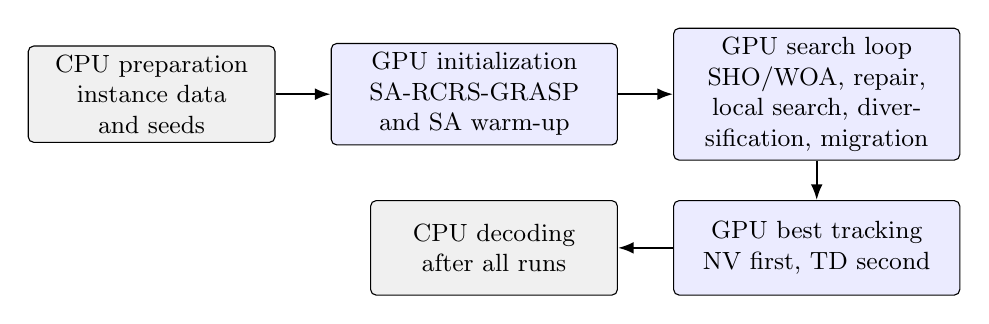
\begin{tikzpicture}[font=\small, node distance=5mm and 7mm,
  box/.style={draw, rounded corners=2pt, align=center, minimum height=12mm, text width=29mm},
  gpu/.style={draw, rounded corners=2pt, align=center, fill=blue!8, minimum height=12mm, text width=34mm},
  flow/.style={-{Latex[length=2mm]}, thick}]
\node[box, fill=gray!12] (prep) {CPU preparation\\instance data and seeds};
\node[gpu, right=of prep] (init) {GPU initialization\\SA-RCRS-GRASP and SA warm-up};
\node[gpu, right=of init] (search) {GPU search loop\\SHO/WOA, repair, local search, diversification, migration};
\node[gpu, below=of search] (best) {GPU best tracking\\NV first, TD second};
\node[box, fill=gray!12, left=of best] (decode) {CPU decoding\\after all runs};
\draw[flow] (prep) -- (init);
\draw[flow] (init) -- (search);
\draw[flow] (search) -- (best);
\draw[flow] (best) -- (decode);
\end{tikzpicture}
\caption{Full-GPU PH-SHOWOA workflow. The GPU search and best-tracking kernels repeat for each generation; the search state remains on the GPU during a run. CPU--GPU transfer occurs only for preparation and final decoding.}
\label{fig:workflow}
\end{figure}

\section{Results}\label{sec:results}

\subsection{Experimental configurations and evaluation metrics}\label{sec:experiments}

The comparison uses the Python PH-SHOWOA implementation as the reference and the fullGPU-SA-RCRS-GRASP Python implementation as the proposed method. For each instance, we report NV, TD, and average runtime per run. The stored results should be accompanied in the final submission by the exact GPU model, CPU model, RAM, CUDA/Numba versions, population size, iteration limit, number of runs, and random-seed policy. These details are necessary for a reproducible runtime comparison.

The reported quality values are compared in the original NV-first order: NV first and TD second. Runtime speedup is calculated as $t_{\mathrm{PH\mbox{-}SHOWOA}}/t_{\mathrm{GPU}}$. Because the two implementations use randomized search, future experiments should run both methods with the same seed set and report mean and standard deviation or confidence intervals. The current table is therefore an empirical performance record, not a statistical significance claim.

\subsection{Model performance analysis}\label{sec:performance}

Table~\ref{tab:results} presents the supplied results. The full-GPU method uses the same NV as the reference on 14 of 15 instances and reduces NV from 14 to 13 on Rdp103. It obtains equal or lower TD on 14 instances; Rdp103 is the only case with a larger TD because the proposed method uses one fewer vehicle. Under the NV-first objective of the original paper, this is an improvement because the vehicle reduction takes precedence over the distance increase.

The runtime difference is large across all instance sizes. The total of the reported average runtimes is 104,175 s for the reference and 3,648.2 s for fullGPU-SA-RCRS-GRASP, giving an aggregate speedup of 28.6$\times$. Instance speedups range from 20.3$\times$ to 105.3$\times$, with a median of 30.8$\times$. The gain is strongest on the 10-customer instance, while the 100-customer instances still show substantial reductions. The aggregate TD is 15,447.297 for the proposed method and 15,810.510 for the reference, a 2.30\% reduction on this selected set. These results support the claim that keeping the complete search state on the GPU removes important overhead without an obvious loss of routing quality.

\begin{table*}[t]
\centering
\caption{Reported comparison between fullGPU-SA-RCRS-GRASP and the Python PH-SHOWOA reference. Lower NV, TD, and time are better.}
\label{tab:results}
\resizebox{\textwidth}{!}{%
\begin{tabular}{llrrrrrrr}
\toprule
Instance & Size & \multicolumn{3}{c}{fullGPU-SA-RCRS-GRASP} & \multicolumn{3}{c}{PH-SHOWOA reference} & Speedup \\
\cmidrule(lr){3-5}\cmidrule(lr){6-8}
& & NV & TD & Avg./run (s) & NV & TD & Avg./run (s) & ($\times$) \\
\midrule
RCdp1001 & 10 & 3 & 348.980 & 1.70 & 3 & 348.980 & 179 & 105.3 \\
RCdp5001 & 50 & 9 & 994.180 & 27.90 & 9 & 996.350 & 1316 & 47.2 \\
RCdp5007 & 50 & 7 & 811.080 & 29.73 & 7 & 816.880 & 1424 & 47.9 \\
RCdp5004 & 50 & 6 & 733.200 & 31.07 & 6 & 747.470 & 1479 & 47.6 \\
RCdp101 & 100 & 15 & 1670.310 & 121.17 & 15 & 1707.340 & 3229 & 26.6 \\
Cdp103 & 100 & 10 & 932.777 & 121.07 & 10 & 939.220 & 4780 & 39.5 \\
Rcdp205 & 100 & 4 & 1332.860 & 467.20 & 4 & 1427.400 & 10730 & 23.0 \\
Rdp210 & 100 & 3 & 959.980 & 584.60 & 3 & 1033.360 & 17990 & 30.8 \\
Rcdp207 & 100 & 3 & 1108.940 & 483.76 & 3 & 1133.680 & 14114 & 29.2 \\
Rcdp202 & 100 & 4 & 1176.990 & 584.00 & 4 & 1282.590 & 11884 & 20.3 \\
Rdp103 & 100 & 13 & 1382.690 & 152.20 & 14 & 1262.560 & 4084 & 26.8 \\
Cdp104 & 100 & 10 & 897.060 & 120.27 & 10 & 898.900 & 4679 & 38.9 \\
Cdp102 & 100 & 10 & 959.470 & 116.90 & 10 & 997.620 & 4439 & 38.0 \\
Rdp203 & 100 & 3 & 947.060 & 662.90 & 3 & 1006.190 & 19546 & 29.5 \\
Rcdp104 & 100 & 11 & 1191.720 & 143.73 & 11 & 1211.970 & 4302 & 29.9 \\
\bottomrule
\end{tabular}}
\end{table*}

\section{Discussion}\label{sec:discussion}

\subsection{Component interpretation and ablation need}

The observed runtime reduction is consistent with the design of the proposed method. Preallocated device tensors avoid repeated allocation, and the GPU-resident loop avoids copying the population between CPU and GPU at every generation. The SA-RCRS-GRASP initializer adds structured and randomized feasible constructions before the hybrid search begins. However, the current results do not isolate the contribution of each component. A future ablation study should compare the CPU reference, GPU residency alone, GPU residency with RCRS-GRASP, and the complete SA-RCRS-GRASP method under identical seeds and stopping conditions.

\subsection{Comparison with the reference implementation}

Relative to the Python PH-SHOWOA reference, the proposed method retains or improves NV on all 15 reported instances. It also improves or matches TD on 14 instances. The Rdp103 result illustrates the importance of using the original comparison rule: the proposed method uses one fewer vehicle, so its larger TD does not make it worse under the NV-first objective. The result table therefore supports the intended quality priority rather than a distance-only comparison.

\subsection{Practical implications}

The full-GPU design is useful when many independent population members and route operations must be processed repeatedly. Its main practical benefit is shorter wall-clock time, which can allow more runs, larger populations, or additional parameter studies within a fixed computing budget. The GPU workflow is also suitable for experiments where solutions should remain on the device until a final answer is required.

\subsection{Limitations and future prospects}

The present method has limitations that come from its algorithmic scope. First, its fixed-shape route and scratch tensors require preselected bounds for the number of routes and route positions. This design is efficient for the tested instances, but it uses memory proportional to population size and problem size. Very large instances may require a smaller population, a compact encoding, or a different kernel layout. Second, SA-RCRS-GRASP, local-search intervals, stagnation control, and island migration introduce hyperparameters. Their current values are effective for the reported configuration, but their best settings can depend on customer distribution, time-window tightness, and GPU memory capacity. Adaptive parameter control is therefore a useful next step.

The implementation also addresses a static, single-depot VRPSPDTW with deterministic travel times and a homogeneous fleet. It does not yet model real-time requests, uncertain travel times, multiple depots, heterogeneous vehicles, driver regulations, or explicit emissions. Extending the GPU kernels to these operational features is not a simple data-format change because every feasibility and repair operator must be adapted. Future work can evaluate compact tensor encodings, adaptive search control, and dynamic or stochastic extensions while preserving the NV-first decision rule.

\section{Conclusion}\label{sec:conclusion}

This paper presented fullGPU-SA-RCRS-GRASP, a Python CUDA implementation of PH-SHOWOA for VRPSPDTW. The method stores the population and search state as preallocated tensors and performs initialization, SA warm-up, SHO/WOA evolution, route improvement, diversification, migration, and best tracking on the GPU. SA-RCRS-GRASP replaces the original initialization with a construction that balances greediness and diversity. On the supplied 15-instance result set, the method retains or improves NV on every instance, obtains equal or lower TD on 14 instances, and reduces the aggregate reported runtime by 28.6$\times$. Future work will test the complete benchmark under matched seeds and hardware, add statistical tests, and further improve GPU route operators for harder 100-customer instances.

\backmatter

\section*{Declarations}
\subsection*{Data and code availability}
The implementation, benchmark inputs, and experiment scripts are available at \url{https://github.com/Welkie/ph-showoa}. The full-GPU Python implementation is in \texttt{src\_python\_gpu\_SA\_RCRS\_GRASP}. The original PH-SHOWOA study reports that its underlying benchmark data are available from the VRPenstein repository \cite{nguyen2026phshowoa}.
\subsection*{Competing interests}
The authors declare no competing interests.
\subsection*{Funding}
No external funding was received for this study.

\bibliography{sn-bibliography}
\end{document}
